\chapter{Sessioni}
\label{cap:sessioni}

\begin{tcolorbox}[title=Mappa del capitolo]
Obiettivi, Teoria sessioni, Lifecycle, Configurazione sicura, Gestione dati, Security (hijacking/fixation/CSRF), Storage handlers, Esempi pratici, Progetti completi, Troubleshooting, Esercizi, Riferimenti.
\end{tcolorbox}

\section{Obiettivi di apprendimento}

Al termine di questo capitolo sarai in grado di:

\begin{itemize}
    \item Comprendere come funzionano le sessioni HTTP
    \item Avviare e configurare sessioni in modo sicuro
    \item Memorizzare e recuperare dati nelle sessioni
    \item Implementare autenticazione con sessioni
    \item Proteggere le sessioni da session hijacking e fixation
    \item Rigenerare ID sessione nei momenti critici
    \item Gestire logout e scadenza sessioni
    \item Utilizzare session handlers personalizzati
\end{itemize}

\section{Teoria: Cosa Sono le Sessioni}

\subsection{Il Problema dello Stato in HTTP}

HTTP è un protocollo \textbf{stateless} (senza stato): ogni richiesta è indipendente e il server non "ricorda" le richieste precedenti dello stesso client. Questo crea un problema:

\begin{tcolorbox}[colback=orange!10, colframe=orange!60, title=Problema]
Come fa un'applicazione web a ricordare che un utente ha fatto login? Come mantiene il carrello della spesa tra le pagine?
\end{tcolorbox}

Le \textbf{sessioni} risolvono questo problema permettendo di associare dati persistenti a un utente specifico attraverso molteplici richieste HTTP.

\subsection{Sessioni vs Cookie}

\begin{center}
\begin{tabular}{|l|p{5cm}|p{5cm}|}
\hline
\textbf{Aspetto} & \textbf{Cookie} & \textbf{Sessioni} \\
\hline
\textbf{Storage} & Client-side (browser) & Server-side (file/DB) \\
\hline
\textbf{Dimensione} & Limitata (4KB max) & Illimitata (limiti server) \\
\hline
\textbf{Sicurezza} & Visibili/modificabili dall'utente & Protetti lato server \\
\hline
\textbf{Durata} & Persistente (giorni/mesi) & Temporanea (minuti/ore) \\
\hline
\textbf{Uso tipico} & Preferenze UI, tracking & Autenticazione, carrello \\
\hline
\textbf{Traffico rete} & Inviato ad ogni richiesta & Solo ID inviato \\
\hline
\end{tabular}
\end{center}

\begin{nota}
Le sessioni \textbf{usano un cookie} (PHPSESSID) per identificare l'utente, ma i dati effettivi sono memorizzati sul server. Il cookie contiene solo l'ID univoco della sessione.
\end{nota}

\subsection{Come Funzionano le Sessioni PHP}

\begin{enumerate}
    \item Client richiede una pagina PHP
    \item Server chiama \texttt{session\_start()}
    \item PHP controlla se esiste cookie PHPSESSID:
    \begin{itemize}
        \item \textbf{NO}: Crea nuovo session ID, crea file sessione, invia cookie al client
        \item \textbf{SÌ}: Legge session ID dal cookie, carica dati da file sessione
    \end{itemize}
    \item Script accede/modifica \texttt{\$\_SESSION}
    \item Fine script: PHP salva \texttt{\$\_SESSION} nel file di sessione
    \item Richieste successive usano lo stesso session ID per accedere agli stessi dati
\end{enumerate}

\section{Session Lifecycle}

\begin{center}
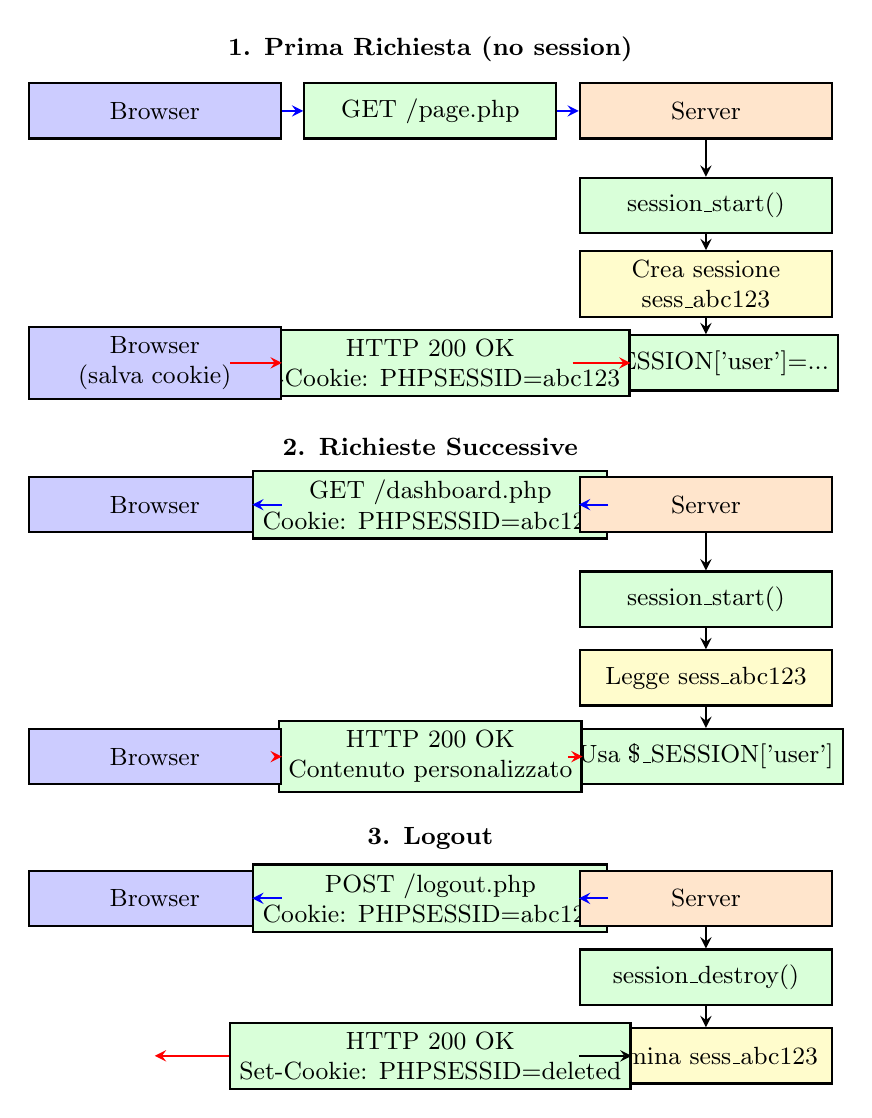
\begin{tikzpicture}[
    node distance=1.2cm,
    box/.style={rectangle, draw, thick, minimum width=3.2cm, minimum height=0.7cm, align=center, font=\small},
    client/.style={box, fill=blue!20},
    server/.style={box, fill=orange!20},
    action/.style={box, fill=green!15},
    storage/.style={box, fill=yellow!20},
    arrow/.style={->, thick, >=stealth}
]
    % Prima richiesta
    \node[above, font=\small\bfseries] at (3.5,7.5) {1. Prima Richiesta (no session)};

    \node[client] (browser1) at (0,7) {Browser};
    \node[action] (req1) at (3.5,7) {GET /page.php};
    \node[server] (server1) at (7,7) {Server};

    \draw[arrow, blue] (browser1) -- (req1);
    \draw[arrow, blue] (req1) -- (server1);

    % Session start
    \node[action] (start) at (7,5.8) {session\_start()};
    \node[storage] (create) at (7,4.8) {Crea sessione\\sess\_abc123};
    \node[action] (setdata) at (7,3.8) {\$\_SESSION['user']=...};

    \draw[arrow] (server1) -- (start);
    \draw[arrow] (start) -- (create);
    \draw[arrow] (create) -- (setdata);

    % Response con Set-Cookie
    \node[action] (response1) at (3.5,3.8) {HTTP 200 OK\\Set-Cookie: PHPSESSID=abc123};
    \node[client] (browser2) at (0,3.8) {Browser\\(salva cookie)};

    \draw[arrow, red] (setdata) -- (response1);
    \draw[arrow, red] (response1) -- (browser2);

    % Seconda richiesta
    \node[above, font=\small\bfseries] at (3.5,2.5) {2. Richieste Successive};

    \node[client] (browser3) at (0,2) {Browser};
    \node[action] (req2) at (3.5,2) {GET /dashboard.php\\Cookie: PHPSESSID=abc123};
    \node[server] (server2) at (7,2) {Server};

    \draw[arrow, blue] (browser3) -- (req2);
    \draw[arrow, blue] (req2) -- (server2);

    % Load session
    \node[action] (start2) at (7,0.8) {session\_start()};
    \node[storage] (load) at (7,-0.2) {Legge sess\_abc123};
    \node[action] (use) at (7,-1.2) {Usa \$\_SESSION['user']};

    \draw[arrow] (server2) -- (start2);
    \draw[arrow] (start2) -- (load);
    \draw[arrow] (load) -- (use);

    % Response
    \node[action] (response2) at (3.5,-1.2) {HTTP 200 OK\\Contenuto personalizzato};
    \node[client] (browser4) at (0,-1.2) {Browser};

    \draw[arrow, red] (use) -- (response2);
    \draw[arrow, red] (response2) -- (browser4);

    % Logout
    \node[above, font=\small\bfseries] at (3.5,-2.5) {3. Logout};

    \node[client] (browser5) at (0,-3) {Browser};
    \node[action] (req3) at (3.5,-3) {POST /logout.php\\Cookie: PHPSESSID=abc123};
    \node[server] (server3) at (7,-3) {Server};

    \draw[arrow, blue] (browser5) -- (req3);
    \draw[arrow, blue] (req3) -- (server3);

    \node[action] (destroy) at (7,-4) {session\_destroy()};
    \node[storage] (delete) at (7,-5) {Elimina sess\_abc123};
    \node[action] (response3) at (3.5,-5) {HTTP 200 OK\\Set-Cookie: PHPSESSID=deleted};

    \draw[arrow] (server3) -- (destroy);
    \draw[arrow] (destroy) -- (delete);
    \draw[arrow] (delete) -- (response3);
    \draw[arrow, red] (response3) -- (0,-5);
\end{tikzpicture}
\end{center}

\section{Configurazione Sessioni Sicure}

\subsection{Avvio Sessione Base}

\begin{lstlisting}[language=PHP, caption={Avvio sessione semplice}]
<?php
// SEMPRE prima di qualsiasi output HTML
session_start();

// Ora puoi usare $_SESSION
$_SESSION['username'] = 'mario';
echo "Sessione avviata per: " . $_SESSION['username'];
?>
\end{lstlisting}

\begin{attenzione}
\texttt{session\_start()} DEVE essere chiamato:
\begin{itemize}
    \item Prima di qualsiasi output (HTML, echo, spazi)
    \item In ogni pagina che usa sessioni
    \item Una sola volta per richiesta
\end{itemize}
\end{attenzione}

\subsection{Configurazione Sicura Completa}

\begin{lstlisting}[language=PHP, caption={Configurazione sessioni sicure}]
<?php
// Configurazione PRIMA di session_start()

// Cookie settings sicuri
session_set_cookie_params([
    'lifetime' => 0,              // Session cookie (scade alla chiusura browser)
    'path' => '/',                // Valido per tutto il sito
    'domain' => '',               // Dominio corrente
    'secure' => true,             // Solo HTTPS
    'httponly' => true,           // Non accessibile da JavaScript
    'samesite' => 'Strict'        // Protezione CSRF
]);

// Impostazioni di sicurezza
ini_set('session.use_strict_mode', '1');        // Rifiuta session ID non generati dal server
ini_set('session.cookie_httponly', '1');        // Protezione XSS
ini_set('session.use_only_cookies', '1');       // Non accettare ID da URL
ini_set('session.cookie_samesite', 'Strict');   // Protezione CSRF

// Nome cookie personalizzato (opzionale, migliora sicurezza per oscurità)
session_name('MY_SESSION_ID');

// Avvia sessione
session_start();

// Timeout sessione (30 minuti)
if (isset($_SESSION['LAST_ACTIVITY']) &&
    (time() - $_SESSION['LAST_ACTIVITY'] > 1800)) {
    session_unset();
    session_destroy();
    header('Location: /login.php?timeout=1');
    exit;
}
$_SESSION['LAST_ACTIVITY'] = time();
?>
\end{lstlisting}

\subsection{Rigenerazione Session ID}

\begin{lstlisting}[language=PHP, caption={Rigenerazione ID nei momenti critici}]
<?php
session_start();

// Dopo login SUCCESS
function login_user($user_id) {
    // PRIMA: Rigenera ID per prevenire session fixation
    session_regenerate_id(true);  // true = elimina vecchio file sessione

    // POI: Imposta dati utente
    $_SESSION['user_id'] = $user_id;
    $_SESSION['logged_in'] = true;
    $_SESSION['login_time'] = time();
    $_SESSION['ip_address'] = $_SERVER['REMOTE_ADDR'];
    $_SESSION['user_agent'] = $_SERVER['HTTP_USER_AGENT'];
}

// Dopo cambio privilegi (es. da user a admin)
function elevate_to_admin() {
    session_regenerate_id(true);
    $_SESSION['is_admin'] = true;
}

// Periodicamente (ogni 15 minuti)
if (!isset($_SESSION['CREATED'])) {
    $_SESSION['CREATED'] = time();
} else if (time() - $_SESSION['CREATED'] > 900) {
    session_regenerate_id(true);
    $_SESSION['CREATED'] = time();
}
?>
\end{lstlisting}

\begin{tcolorbox}[colback=blue!10, colframe=blue!60, title=Quando rigenerare session ID]
\begin{itemize}
    \item \textbf{Dopo login}: Previene session fixation
    \item \textbf{Dopo cambio privilegi}: User→Admin, Guest→User
    \item \textbf{Periodicamente}: Ogni 15-30 minuti per sessioni lunghe
    \item \textbf{Prima di operazioni sensibili}: Cambio password, pagamenti
\end{itemize}
\end{tcolorbox}

\section{Gestione Dati Sessione}

\subsection{Memorizzazione Dati}

\begin{lstlisting}[language=PHP, caption={Tipi di dati in sessione}]
<?php
session_start();

// Scalari
$_SESSION['user_id'] = 123;
$_SESSION['username'] = 'mario_rossi';
$_SESSION['is_admin'] = true;

// Array
$_SESSION['permissions'] = ['read', 'write', 'delete'];
$_SESSION['cart'] = [
    'product_1' => ['qty' => 2, 'price' => 29.99],
    'product_5' => ['qty' => 1, 'price' => 149.99]
];

// Oggetti (devono essere serializzabili)
class User {
    public $id;
    public $name;
    public function __construct($id, $name) {
        $this->id = $id;
        $this->name = $name;
    }
}
$_SESSION['user_object'] = new User(123, 'Mario');

// Dati temporanei (flash messages)
$_SESSION['flash_message'] = 'Operazione completata con successo!';
?>
\end{lstlisting}

\subsection{Lettura Sicura Dati}

\begin{lstlisting}[language=PHP, caption={Accesso sicuro a dati sessione}]
<?php
session_start();

// Verifica esistenza con isset
if (isset($_SESSION['user_id'])) {
    $user_id = $_SESSION['user_id'];
} else {
    // Reindirizza al login
    header('Location: /login.php');
    exit;
}

// Operatore null coalescing (??)
$username = $_SESSION['username'] ?? 'Guest';
$is_admin = $_SESSION['is_admin'] ?? false;

// Validazione tipo
function get_user_id() {
    if (!isset($_SESSION['user_id'])) {
        return null;
    }

    $user_id = $_SESSION['user_id'];

    // Valida che sia un intero positivo
    if (!is_numeric($user_id) || $user_id <= 0) {
        // Sessione compromessa!
        session_destroy();
        return null;
    }

    return (int)$user_id;
}

// Flash messages (mostra una volta, poi rimuovi)
function get_flash_message() {
    $message = $_SESSION['flash_message'] ?? null;
    unset($_SESSION['flash_message']);
    return $message;
}
?>
\end{lstlisting}

\subsection{Rimozione Dati}

\begin{lstlisting}[language=PHP, caption={Rimuovere dati da sessione}]
<?php
session_start();

// Rimuovi singola variabile
unset($_SESSION['cart']);

// Rimuovi tutte le variabili (ma mantieni sessione attiva)
session_unset();  // equivale a $_SESSION = []

// Distruggi sessione completamente
session_destroy();

// Elimina anche il cookie
setcookie(session_name(), '', time() - 3600, '/');
?>
\end{lstlisting}

\section{Sicurezza Sessioni}

\subsection{Session Hijacking (Dirottamento)}

\textbf{Attacco}: Un attaccante ruba il session ID di una vittima e lo usa per impersonarla.

\textbf{Vettori di attacco}:
\begin{itemize}
    \item XSS: JavaScript ruba cookie (\texttt{document.cookie})
    \item Network sniffing: Intercettazione traffico HTTP
    \item Session ID in URL: \texttt{/page.php?PHPSESSID=abc123}
\end{itemize}

\textbf{Protezioni}:

\begin{lstlisting}[language=PHP, caption={Protezione da session hijacking}]
<?php
session_start();

// 1. HttpOnly cookie (previene accesso JavaScript)
ini_set('session.cookie_httponly', '1');

// 2. Secure cookie (solo HTTPS)
ini_set('session.cookie_secure', '1');

// 3. Valida IP e User-Agent (OPZIONALE, problemi con proxy)
function validate_session() {
    // Verifica IP
    if (isset($_SESSION['ip_address'])) {
        if ($_SESSION['ip_address'] !== $_SERVER['REMOTE_ADDR']) {
            session_destroy();
            die('Session hijacking detected!');
        }
    } else {
        $_SESSION['ip_address'] = $_SERVER['REMOTE_ADDR'];
    }

    // Verifica User-Agent
    if (isset($_SESSION['user_agent'])) {
        if ($_SESSION['user_agent'] !== $_SERVER['HTTP_USER_AGENT']) {
            session_destroy();
            die('Session hijacking detected!');
        }
    } else {
        $_SESSION['user_agent'] = $_SERVER['HTTP_USER_AGENT'];
    }
}

validate_session();
?>
\end{lstlisting}

\begin{attenzione}
Validare IP può causare problemi con:
\begin{itemize}
    \item Utenti mobile (IP cambia tra WiFi e 4G)
    \item Proxy/Load balancer aziendali
    \item VPN che ruotano IP
\end{itemize}
Valuta se il tuo caso d'uso lo richiede.
\end{attenzione}

\subsection{Session Fixation}

\textbf{Attacco}: L'attaccante forza la vittima a usare un session ID conosciuto dall'attaccante.

\textbf{Scenario}:
\begin{enumerate}
    \item Attaccante ottiene session ID: \texttt{PHPSESSID=malicious123}
    \item Attaccante invia link alla vittima: \texttt{http://site.com/?PHPSESSID=malicious123}
    \item Vittima fa login usando quel session ID
    \item Attaccante usa \texttt{malicious123} per accedere come la vittima
\end{enumerate}

\textbf{Protezioni}:

\begin{lstlisting}[language=PHP, caption={Protezione da session fixation}]
<?php
// 1. Use strict mode (rifiuta ID non generati dal server)
ini_set('session.use_strict_mode', '1');

// 2. Accetta ID SOLO da cookie (non da GET/POST)
ini_set('session.use_only_cookies', '1');

// 3. RIGENERA ID dopo login
function secure_login($username, $password) {
    // Verifica credenziali
    $user = authenticate($username, $password);

    if ($user) {
        // RIGENERA ID PRIMA di impostare dati sensibili
        session_regenerate_id(true);

        $_SESSION['user_id'] = $user['id'];
        $_SESSION['logged_in'] = true;

        return true;
    }

    return false;
}
?>
\end{lstlisting}

\subsection{CSRF con Sessioni}

Anche con sessioni sicure, sei vulnerabile a CSRF. Usa token CSRF:

\begin{lstlisting}[language=PHP, caption={CSRF protection con sessioni}]
<?php
session_start();

// Genera token CSRF
function generate_csrf_token() {
    if (!isset($_SESSION['csrf_token'])) {
        $_SESSION['csrf_token'] = bin2hex(random_bytes(32));
    }
    return $_SESSION['csrf_token'];
}

// Verifica token CSRF
function verify_csrf_token($token) {
    return isset($_SESSION['csrf_token']) &&
           hash_equals($_SESSION['csrf_token'], $token);
}

// Form HTML
$csrf_token = generate_csrf_token();
?>
<form method="POST" action="/transfer.php">
    <input type="hidden" name="csrf_token" value="<?= htmlspecialchars($csrf_token) ?>">
    <input type="text" name="amount">
    <button type="submit">Transfer</button>
</form>

<?php
// transfer.php
session_start();

if ($_SERVER['REQUEST_METHOD'] === 'POST') {
    $token = $_POST['csrf_token'] ?? '';

    if (!verify_csrf_token($token)) {
        die('CSRF attack detected!');
    }

    // Processa trasferimento in sicurezza
    process_transfer($_POST['amount']);
}
?>
\end{lstlisting}

\section{Logout Sicuro}

\begin{lstlisting}[language=PHP, caption={Logout completo e sicuro}]
<?php
// logout.php
session_start();

// 1. Cancella tutte le variabili di sessione
$_SESSION = [];

// 2. Elimina il cookie di sessione
if (isset($_COOKIE[session_name()])) {
    $params = session_get_cookie_params();
    setcookie(
        session_name(),
        '',
        time() - 42000,
        $params['path'],
        $params['domain'],
        $params['secure'],
        $params['httponly']
    );
}

// 3. Distruggi la sessione lato server
session_destroy();

// 4. Rigenera session ID (per sicurezza)
session_start();
session_regenerate_id(true);

// 5. Reindirizza al login
header('Location: /login.php?logout=success');
exit;
?>
\end{lstlisting}

\section{Esempio Completo: Sistema Autenticazione}

\begin{lstlisting}[language=PHP, caption={config.php - Configurazione}]
<?php
// config.php
function init_secure_session() {
    // Configurazione cookie
    session_set_cookie_params([
        'lifetime' => 0,
        'path' => '/',
        'domain' => '',
        'secure' => isset($_SERVER['HTTPS']),
        'httponly' => true,
        'samesite' => 'Strict'
    ]);

    // Impostazioni sicurezza
    ini_set('session.use_strict_mode', '1');
    ini_set('session.cookie_httponly', '1');
    ini_set('session.use_only_cookies', '1');
    ini_set('session.cookie_samesite', 'Strict');

    session_start();

    // Timeout 30 minuti
    if (isset($_SESSION['LAST_ACTIVITY']) &&
        (time() - $_SESSION['LAST_ACTIVITY'] > 1800)) {
        session_unset();
        session_destroy();
        session_start();
        $_SESSION['timeout'] = true;
    }
    $_SESSION['LAST_ACTIVITY'] = time();

    // Rigenera periodicamente
    if (!isset($_SESSION['CREATED'])) {
        $_SESSION['CREATED'] = time();
    } else if (time() - $_SESSION['CREATED'] > 900) {
        session_regenerate_id(true);
        $_SESSION['CREATED'] = time();
    }
}

function is_logged_in() {
    return isset($_SESSION['user_id']) && $_SESSION['logged_in'] === true;
}

function require_login() {
    if (!is_logged_in()) {
        header('Location: /login.php');
        exit;
    }
}

function get_user_id() {
    return $_SESSION['user_id'] ?? null;
}
?>
\end{lstlisting}

\begin{lstlisting}[language=PHP, caption={login.php - Pagina login}]
<?php
// login.php
require 'config.php';
init_secure_session();

$error = null;

if ($_SERVER['REQUEST_METHOD'] === 'POST') {
    $username = $_POST['username'] ?? '';
    $password = $_POST['password'] ?? '';

    // Connessione DB (esempio)
    $pdo = new PDO('mysql:host=localhost;dbname=app', 'user', 'pass');

    // Query preparata
    $stmt = $pdo->prepare('SELECT id, password_hash FROM users WHERE username = ?');
    $stmt->execute([$username]);
    $user = $stmt->fetch();

    if ($user && password_verify($password, $user['password_hash'])) {
        // Login SUCCESS
        session_regenerate_id(true);  // Previene session fixation

        $_SESSION['user_id'] = $user['id'];
        $_SESSION['logged_in'] = true;
        $_SESSION['login_time'] = time();

        header('Location: /dashboard.php');
        exit;
    } else {
        $error = 'Username o password errati';
    }
}
?>
<!DOCTYPE html>
<html>
<head>
    <title>Login</title>
</head>
<body>
    <h1>Login</h1>

    <?php if ($error): ?>
        <div class="error"><?= htmlspecialchars($error) ?></div>
    <?php endif; ?>

    <?php if (isset($_SESSION['timeout'])): ?>
        <div class="warning">Sessione scaduta. Effettua nuovamente il login.</div>
        <?php unset($_SESSION['timeout']); ?>
    <?php endif; ?>

    <form method="POST">
        <label>Username: <input type="text" name="username" required></label><br>
        <label>Password: <input type="password" name="password" required></label><br>
        <button type="submit">Login</button>
    </form>
</body>
</html>
\end{lstlisting}

\begin{lstlisting}[language=PHP, caption={dashboard.php - Area riservata}]
<?php
// dashboard.php
require 'config.php';
init_secure_session();
require_login();  // Reindirizza se non loggato

$user_id = get_user_id();

// Carica dati utente
$pdo = new PDO('mysql:host=localhost;dbname=app', 'user', 'pass');
$stmt = $pdo->prepare('SELECT username, email FROM users WHERE id = ?');
$stmt->execute([$user_id]);
$user = $stmt->fetch();
?>
<!DOCTYPE html>
<html>
<head>
    <title>Dashboard</title>
</head>
<body>
    <h1>Benvenuto, <?= htmlspecialchars($user['username']) ?></h1>

    <p>Email: <?= htmlspecialchars($user['email']) ?></p>

    <p>Loggato da:
        <?= htmlspecialchars(date('H:i:s', $_SESSION['login_time'])) ?>
    </p>

    <a href="/logout.php">Logout</a>
</body>
</html>
\end{lstlisting}

\section{Troubleshooting Sessioni}

\subsection{Errore: "Headers already sent"}

\begin{lstlisting}[language=PHP]
Warning: session_start(): Cannot send session cookie - headers already sent
\end{lstlisting}

\textbf{Causa}: Output HTML/spazi prima di \texttt{session\_start()}.

\textbf{Soluzione}:
\begin{itemize}
    \item Metti \texttt{session\_start()} come PRIMA istruzione
    \item Nessuno spazio/newline prima di \texttt{<?php}
    \item Nessun \texttt{echo} o HTML prima
    \item Verifica BOM in UTF-8 (usa UTF-8 without BOM)
\end{itemize}

\subsection{Sessione Non Persiste}

\textbf{Possibili cause}:
\begin{itemize}
    \item Cookie disabilitati nel browser
    \item Path cookie errato
    \item Domain cookie non corretto
    \item Permessi directory sessioni (di solito \texttt{/tmp})
\end{itemize}

\textbf{Debug}:
\begin{lstlisting}[language=PHP]
<?php
session_start();

echo "Session ID: " . session_id() . "<br>";
echo "Session Name: " . session_name() . "<br>";
echo "Session Save Path: " . session_save_path() . "<br>";
echo "Cookie Params: ";
print_r(session_get_cookie_params());

$_SESSION['test'] = 'value';
echo "<br>Session Data: ";
print_r($_SESSION);
?>
\end{lstlisting}

\subsection{Sessioni su Server Condiviso}

Su hosting condiviso, directory sessioni è condivisa. Usa directory personalizzata:

\begin{lstlisting}[language=PHP]
<?php
$custom_path = __DIR__ . '/sessions';

// Crea directory se non esiste
if (!is_dir($custom_path)) {
    mkdir($custom_path, 0700, true);
}

session_save_path($custom_path);
session_start();
?>
\end{lstlisting}

\section{Esercizi}

\subsection{Esercizio 1 (Base)}

Crea un sistema di login semplice con:
\begin{itemize}
    \item Pagina login.php con form
    \item Validazione username/password hardcoded
    \item Sessione che memorizza username
    \item Pagina dashboard.php accessibile solo se loggati
    \item Logout che invalida sessione
\end{itemize}

\subsection{Esercizio 2 (Intermedio)}

Estendi l'esercizio 1 aggiungendo:
\begin{itemize}
    \item Timeout sessione dopo 10 minuti di inattività
    \item Messaggio flash "Login effettuato con successo"
    \item Contatore numero di pagine visitate nella sessione
    \item Log timestamp ultimo accesso
\end{itemize}

\subsection{Esercizio 3 (Avanzato)}

Crea sistema autenticazione sicuro con:
\begin{itemize}
    \item Database MySQL con tabella users (username, password\_hash, email)
    \item Registrazione con password hashing (password\_hash)
    \item Login con rigenerazione session ID
    \item Protezione CSRF su tutti i form
    \item Validazione IP e User-Agent
    \item Logout completo
\end{itemize}

\section{Progetto: Carrello E-commerce}

Implementa un carrello della spesa con sessioni:

\textbf{Funzionalità richieste}:
\begin{itemize}
    \item Aggiungi prodotto al carrello (ID, quantità, prezzo)
    \item Visualizza carrello con totale
    \item Aggiorna quantità prodotto
    \item Rimuovi prodotto
    \item Svuota carrello
    \item Carrello persiste tra le pagine
    \item Timeout carrello dopo 1 ora
\end{itemize}

\textbf{Sicurezza}:
\begin{itemize}
    \item Valida ID prodotto (esiste nel DB)
    \item Valida quantità (> 0, < 100)
    \item Valida prezzo lato server (non fidarsi del client)
    \item Protezione CSRF
\end{itemize}

\section{Verifica}

\begin{enumerate}
    \item Qual è la differenza tra cookie e sessioni?
    \item Perché è importante rigenerare session ID dopo login?
    \item Cosa fa \texttt{session\_regenerate\_id(true)}? Cosa significa il parametro \texttt{true}?
    \item Quali sono i tre flag di sicurezza principali per cookie di sessione?
    \item Come si protegge da session fixation?
    \item Come si protegge da session hijacking?
    \item Quando usare \texttt{session\_unset()} vs \texttt{session\_destroy()}?
    \item Perché \texttt{session\_start()} deve essere la prima istruzione?
\end{enumerate}

\section{Best Practices Riepilogo}

\begin{tcolorbox}[colback=green!10, colframe=green!60, title=Checklist Sessioni Sicure]
\begin{itemize}
    \item[$\square$] \texttt{session\_start()} come prima istruzione
    \item[$\square$] Cookie con HttpOnly, Secure, SameSite
    \item[$\square$] \texttt{use\_strict\_mode} = 1
    \item[$\square$] \texttt{use\_only\_cookies} = 1
    \item[$\square$] Rigenerare ID dopo login
    \item[$\square$] Rigenerare ID dopo cambio privilegi
    \item[$\square$] Timeout sessione (30 minuti)
    \item[$\square$] Logout completo (unset + destroy + cookie delete)
    \item[$\square$] Protezione CSRF con token
    \item[$\square$] Solo HTTPS in produzione
    \item[$\square$] Non memorizzare password in sessione
    \item[$\square$] Validare dati sessione (tipo, range)
\end{itemize}
\end{tcolorbox}

\section{Riferimenti}

\begin{itemize}
    \item PHP Manual - Sessions: \url{https://www.php.net/manual/en/book.session.php}
    \item OWASP Session Management Cheat Sheet: \url{https://cheatsheetseries.owasp.org/cheatsheets/Session_Management_Cheat_Sheet.html}
    \item PHP: The Right Way - Security: \url{https://phptherightway.com/#security}
\end{itemize}
